Le but de cette analyse multi-critère est de déterminer la meilleure solution
parmis les 8 solutions proposées dans la matrice des jugements qui nous a été
donnée. \\

Comme nous souhaitons faire émerger une solution unique, la meilleure (et non
pas classer les solutions les unes par rapport aux autres) grâce aux critères
qui ont été retenus, nous allons utiliser la méthode de détermination Electre
1. \\

Dans un premier temps dans cette analyse multi-critère, nous avons considéré
que tous les critères étaient de même poids. \\

Nous avons ainsi calculé les matrices de concordance et de discordance
relatives à la matrice de jugement. \\
\begin{figure}
    \begin{center}
        \begin{tabular}{|c c c c c|}
            0&3&3&2&3\\
            1&0&2&2&2\\
            2&2&0&2&3\\
            2&3&2&0&3\\
            2&2&3&1&0\\
        \end{tabular}
        \caption{Matrice de concordance (x4)}
    \end{center}
\end{figure}

\begin{figure}
    \begin{center}
        \begin{tabular}{|c c c c c|}
            10&4&2&4&2\\
            2&10&3&6&1\\
            3&4&10&5&2\\
            3&7&3&10&5\\
            3&3&2&5&10\\
        \end{tabular}
        \caption{Matrice de discordance (x10)}
    \end{center}
\end{figure}

Nous avons par la suite testé différentes solutions que voici : \\

On fait varier les seuils de surclassement ainsi que : \\
\begin{figure}
    \begin{center}
        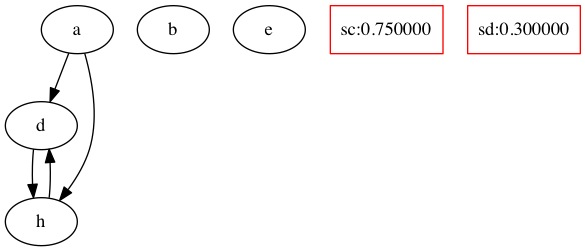
\includegraphics[scale=0.6]{partie3/graph_3_4_3_10.jpeg}
        \caption{Graphe de surclassement : sc = 3/4, sd = 3/10}
    \end{center}
\end{figure}

Avec un seuil de concordance de 3/4 et un seuil de discordance de 3/10, on peut
voir qu’il reste de nombreux liens à faire et donc que les seuils qui ont été
pris sont trop restrictifs. \\

\begin{figure}
    \begin{center}
        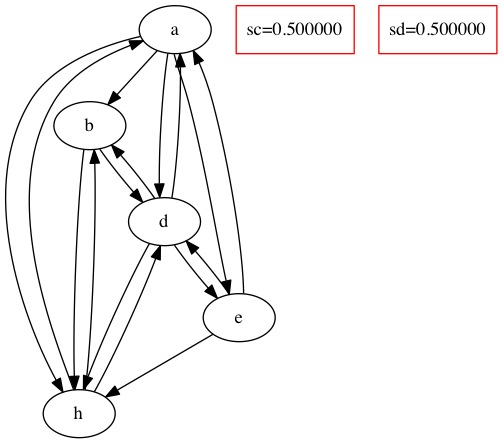
\includegraphics[scale=0.5]{partie3/graph_2_4_5_10.jpeg}
        \caption{Graphe de surclassement : sc = 5/4, sd = 5/10}
    \end{center}
\end{figure}

En prenant un seuil de concordance de 2/4 et un seuil de discordance de 5/10,
on peut voir à l’inverse que trop de liens ont été créés, et la situation est
inexploitable. Nous avons donc choisi des critères trop souples. \\

\begin{figure}
    \begin{center}
        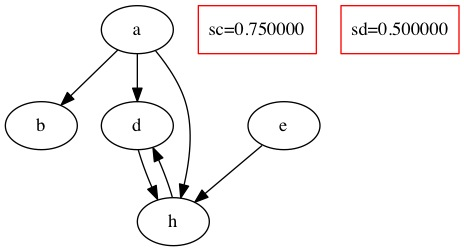
\includegraphics[scale=0.7]{partie3/graph_3_4_5_10.jpeg}
        \caption{Graphe de surclassement : sc = 3/4, sd = 5/10}
    \end{center}
\end{figure}

En prenant un seuil de concordance de 3/4 et un seuil de discordance de 5/10,
on obtient un résultat plus correct cependant elle n’est pas exploitable car
aucune solution ne se dégage clairement, notamment A et E. L’analyse sans
pondération ne suffit donc pas, il va falloir aller plus loin et refaire la
même démarche d’analyse approfondie. \\

Nous allons donc recommencer l’analyse en donnant les poids suivants aux critères : \\
\begin{itemize}
    \item g1 (bénéfice) est de poids 4.
    \item g2 (gestion du stock) est de poids 1.
    \item g3 (équilibre commercial) est de poids 2.
    \item g4 (utilisation des machines 1 et 5) est de poids 2.
\end{itemize}

On met également en place de nouvelles échelles de jugement. \\
Les notes iront de 0 à 10 pour un poids fort (g1), de 2 à 8 pour un poids moyen
(g3 et g4) et de 3 à 7 pour un poids faible (g2). \\

Nous effectuons donc un changement d’échelle sur les notes de la matrice de
jugement : \\
Avec $x\in[a1,b1]$ l’élément de la matrice de jugement dans l’ancienne échelle. \\
~~~~~$y\in[a2,b2]$ l’élément de la matrice de jugement dans la nouvelle échelle. \\
$y = x\cdot(b2-a2)/(b1-a1) + (a2\cdot b1-a1\cdot b2)/(b1-a1)$

De poids fort à poids moyen : $y = x\cdot(8-2)/10 + (2\cdot 10-0)/10 = 0.6\cdot x + 2$ \\
De poids fort à poids faible :$y = x\cdot(7-3)/10 + (3\cdot 10-0)/10 = 0.4\cdot x+ 3$ \\

Cette transformation donne la nouvelle matrice de jugement : \\
\begin{figure}
    \begin{center}
        \begin{tabular}{|c c c c|}
            6&5&5&5\\
            5&4.6&7.4&3.8\\
            3&5.8&5&4.4\\
            5&5.4&3.2&7.4\\
            3&5&6.2&4.4\\
        \end{tabular}
        \caption{Nouvelle matrice de jugement}
    \end{center}
\end{figure}

Nous pouvons calculer les nouvelles matrices de concordance et de discordance : \\
\begin{figure}
    \begin{center}
        \begin{tabular}{|c c c c c|}
            0&7&8&6&7\\
            2&0&6&6&7\\
            3&3&0&3&7\\
            3&6&6&0&7\\
            3&3&8&2&0\\
        \end{tabular}
        \caption{Matrice de concordance (x9)}
    \end{center}
\end{figure}

\begin{figure}
    \begin{center}
        \begin{tabular}{|c c c c c|}
            10&2.4&0.8&2.4&1.2\\
            1.2&10&1.2&3.6&0.6\\
            3&2.4&10&3&1.2\\
            1.8&2.4&1.8&10&3\\
            3&2&0.8&3&10\\
        \end{tabular}
        \caption{Matrice de discordance (x10)}
    \end{center}
\end{figure}

Nous testons une nouvelle fois différentes solutions : \\
\begin{figure}
    \begin{center}
        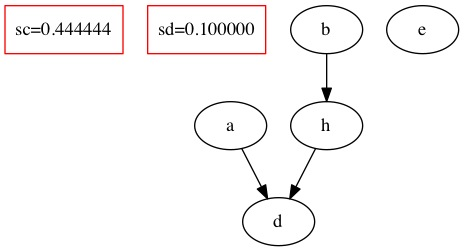
\includegraphics[scale=0.7]{partie3/graph_4_9_1_10.jpeg}
        \caption{Graphe de surclassement : sc = 4/9, sd = 1/10}
    \end{center}
\end{figure}

Comme lors de la première analyse, nous avons pris des seuils trop
contraignants avec un seuil de concordance de 4/9 et un seuil de discordance de
1/10. \\

\begin{figure}
    \begin{center}
        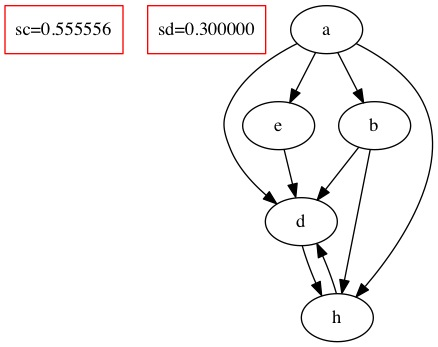
\includegraphics[scale=0.7]{partie3/graph_5_9_3_10.jpeg}
        \caption{Graphe de surclassement : sc = 5/9, sd = 3/10}
    \end{center}
\end{figure}

Lorsque nous choisissons un seuil de concordance de 5/9 et un seuil de
discordance de 3/10, nous arrivons à une solution concluante. \\

L’analyse approfondie met en évidence que la solution A domine au final la
solution E (avec les pondérations que nous avons retenues), et en même temps
domine toutes les autres. \\
La solution que nous retenons dans cette analyse multi-critère est donc la solution A. \\
